\let\negmedspace\undefined
\let\negthickspace\undefined
\documentclass[journal]{IEEEtran}
\usepackage[a5paper, margin=10mm, onecolumn]{geometry}
%\usepackage{lmodern} % Ensure lmodern is loaded for pdflatex
\usepackage{tfrupee} % Include tfrupee package

\setlength{\headheight}{1cm} % Set the height of the header box
\setlength{\headsep}{0mm}     % Set the distance between the header box and the top of the text

\usepackage{gvv-book}
\usepackage{gvv}
\usepackage{cite}
\usepackage{amsmath,amssymb,amsfonts,amsthm}
\usepackage{algorithmic}
\usepackage{graphicx}
\usepackage{textcomp}
\usepackage{xcolor}
\usepackage{txfonts}
\usepackage{listings}
\usepackage{enumitem}
\usepackage{mathtools}
\usepackage{gensymb}
\usepackage{comment}
\usepackage[breaklinks=true]{hyperref}
\usepackage{tkz-euclide} 
\usepackage{listings}
% \usepackage{gvv}                                        
\def\inputGnumericTable{}                                 
\usepackage[latin1]{inputenc}                                
\usepackage{color}                                            
\usepackage{array}                                            
\usepackage{longtable}                                       
\usepackage{calc}                                             
\usepackage{multirow}                                         
\usepackage{hhline}                                           
\usepackage{ifthen}                                           
\usepackage{lscape}
\usepackage{tikz}
\usepackage{textcomp}
\usetikzlibrary{circuits.ee.IEC, positioning}
\begin{document}

\bibliographystyle{IEEEtran}
\vspace{3cm}

\title{9.7.18}
\author{Manognya Kundarapu - EE24BTECH11037
}
% \maketitle
% \newpage
% \bigskip
{\let\newpage\relax\maketitle}

\renewcommand{\thefigure}{\theenumi}
\renewcommand{\thetable}{\theenumi}
\setlength{\intextsep}{10pt} % Space between text and floats


\numberwithin{equation}{enumi}
\numberwithin{figure}{enumi}
\renewcommand{\thetable}{\theenumi}
\textbf{Question:} $e^x dy+\brak{ye^x+2x}dx=0$\\

\begin{enumerate}
    \item \textbf{Theoretical Solution:}\\ 
    \begin{align}
    \frac{dy}{dx}=\frac{-\brak{ye^x+2x}}{e^x}\\
    \frac{dy}{dx}=-y-\frac{2x}{e^x}\\
    \implies \frac{dy}{dx}+y=\frac{2x}{e^x}\\
    \text{Now, it is in the form of linear differential equation;}\\
    \frac{dy}{dx}+y.p\brak{x}=q\brak{x}\\
    \text{Integrating factor,} I.F=e^{\int1.dx}\\
    \implies I.F=e^x\\
    y.e^x=\int\frac{-2x}{e^x}.e^x dx\\
    y.e^x=-x^2+c\\
    \implies y=\frac{-x^2+c}{e^x}\\
    \text{Taking $x_0=0, y_0=1$}\implies k=1\\
    \therefore \text{The final solution is $\frac{-x^2+1}{e^x}$}
    \end{align}
    \item \textbf{Using Method of Finite Differences:}\\ The Method of finite Differences is a numerical technique used to approximate solutions to differential equations.\\We know that;\\
    \begin{align}
        \lim_{x\to 0}\frac{y\brak{x+h}-y\brak{x}}{h}=\frac{dy}{dx}\\
        \approx \frac{y_{n+1}-y_n}{h}=-y-\frac{2x}{e^x}\\
        \implies y_{n+1}=y_n+h\brak{-y_n-\frac{2x_n}{e^{x_n}}}\\
    \end{align}
    Now the following steps were used:
    \begin{enumerate}
        \item Initialized $x_0=0$ and $y_0=1$.
        \item h was taken to be $0.001$, a small value and number of iterations was taken to be $1000$ to ensure accuracy.
        \item Now the subsequent points of the curve were generated through iterations by using the below equations;
        \begin{align}
            x_{n+1}=x_n+h\\
            y_{n+1}=y_n+h\brak{-y_n-\frac{2x_n}{e^{x_n}}}
        \end{align}
    \end{enumerate}
    The below graph shows the comparison between the curve that is obtained theoretically and the simulation curve(numerically generated points through iterations).
\end{enumerate}
\begin{figure}[htbp]
  \centering
  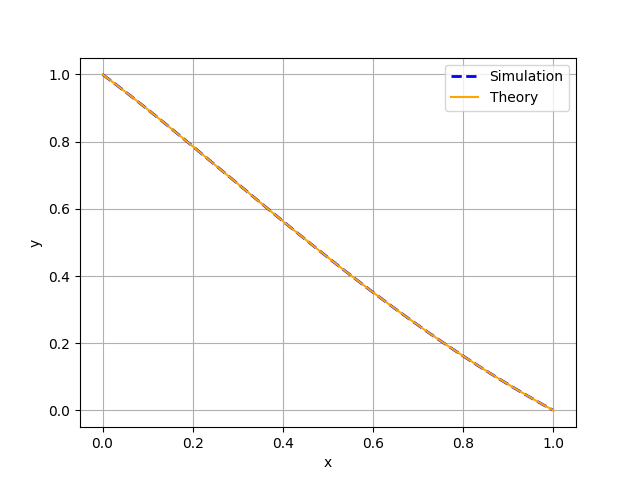
\includegraphics[width=\columnwidth]{figs/curve.png}
\end{figure}

\end{document}
  
